\chapter{Results and discussions}
\section{Introduction}
In this chapter, the results of the experimental tests conducted during this study are concisely presented and discussed. The variation and correlation observed are also presented. This chapter builds from the experimental method (chapter 4).  Four tests were conducted as shown in previous chapter, this was done to validate the objectives of the present study, which is to investigate the effect of HDPE, mild steel and stainless steel on AFFF solution. 
To begin with, the FTIR results were analysed to deduce the functional groups of AFFF solution. The TEM was used to determine the overall size and shape of the particles, DLS was used to determine the particle size distribution and lastly ICP was used to identify the elemental composition of AFFF solution.  

\section{AFFF solution Infrared spectroscopy}
Figure \ref{ch5:figure:spectra} and \ref{ch5:figure:materials} shows the FTIR spectra of the Pure AFFF solution compared to AFFF solution that has been exposed to the materials of interest.  Their functionality in terms of stability, oxidation and reactivity was revealed. Unsurprisingly, most of the chemical and functional groups appear within the group frequency of wavenumber 4000-1500 cm$^{-1}$.
Referring to Figure \ref{ch5:figure:spectra} it can be observed that at the single bond region a broad band appears at 3355 cm$^{-1}$, which has been associated with hydroxy group, H-bonded OH stretch [ref 4]. This functional group is responsible for enhancing the AFFF solution to dissolve in water[ref1].  Medial alkyne C$\equiv$C stretch appears as a weak band at 2120 cm$^{-1}$, this is a vital distinguishing tool since very few organic compound reveal an abortion in this region [ref 3]. The medium band detected at 1637 cm$^{-1}$ can be assigned to Alkenyl C=C stretch vibration. Interestingly, the fingerprint region also revealed quite a few functional groups. However, the Methylene C-H bend and Skeletal C-C vibrations can be disregarded since they appear in most organic compounds. The fluoro compounds, C-F stretch at 1083 cm$^{-1}$ confirms the presence of fluorosurfactant in AFFF concentrate. 
Referring to Figure \ref{ch5:figure:materials}, which compares the FTIR spectra of pure AFFF solution with AFFF solution that has been exposed materials of interest to deduce the significant shifts of functional groups. In the single bond region, a hydroxy group, H-bonded OH stretch still appears in all the FTIR spectra. However, there is a strange absorption peak of aldehyde C-C stretching which appears in AFFF solution (HDPE and Stainless steel exposed) at bands 2710 cm$^{-1}$  and 2697 cm$^{-1}$ respectively[ref. This may indicate an interaction between the AFFF solution and two materials (HDPE and Stainless steel). Moreover, there is a significant shift which can be observed on the triple bond region at bands 2056 cm$^{-1}$ and 2060 cm$^{-1}$ for exposed HDPE and Stainless steel AFFF solution respectively. Consequently, this shift confirms the presence of isothiocyanate N=C=S stretching, which is a very unusual functional group, especially in organic compounds.
It can be clearly observed that there are minor shifts in the functional groups. However, these minor shifts can be subsequently utilised to predict the reaction of the materials with AFFF solution in a long term. This is a very useful prediction technique, since in the present study these materials were immersed to AFFF solution for only five months. In addition, the major reaction in the real world may probably take years to occur. Figure \ref{ch5:figure:pure_afff_images}-\ref{ch5:figure:hdpe_images} in section 6.3 compare the FTIR spectrum of pure materials (HDPE, Mild steel and Stainless steel) with materials exposed to AFFF solution. This was done to further examine and validate the functional group shifts on the exposed materials of interest.  

\begin{figure}[H]
\centering

\begin{subfigure}{.45\textwidth}
    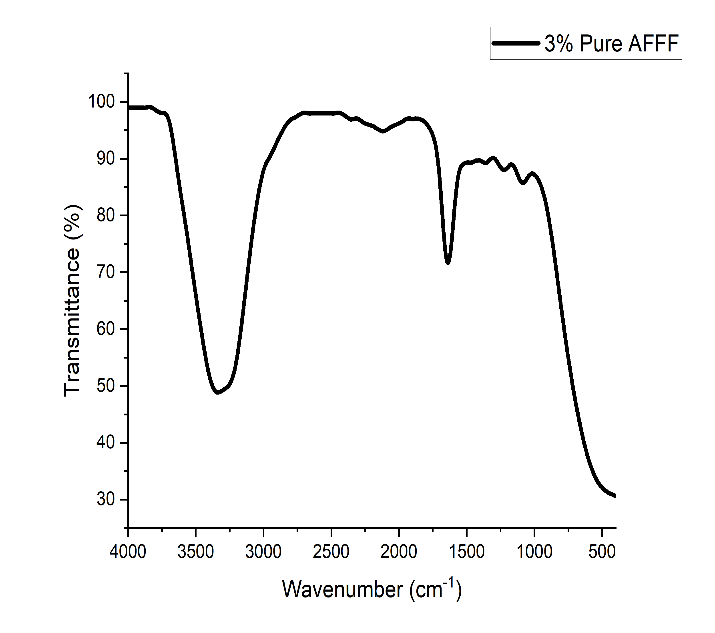
\includegraphics[width=\textwidth]{ftir_spectra.png}
    \caption{}
\end{subfigure}
\begin{subfigure}{.45\textwidth}
    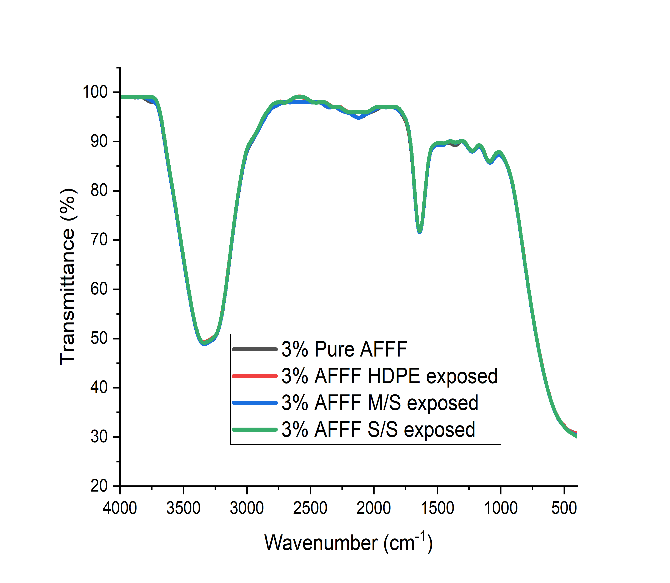
\includegraphics[width=\textwidth]{comparison.png}
    \caption{}
\end{subfigure}

\caption{FTIR spectra, comparison Pure AFFF solution with the AFFF solution that has been exposed to various materials.}
\label{ch5:figure:spectra}
\end{figure}

\section{Infrared spectroscopy of HDPE, Mild steel, and Stainless steel}  
The FTIR spectra of the materials of interest was conducted to substantiate the minor shifts of the functional group on the exposed AFFF solution. Figure \ref{ch5:figure:materials} (a-c) shows the FTIR spectra of the materials of interest. The reactivity of AFFF solution with the materials of interest was the point of interest. It can be observed from Figure \ref{ch5:figure:materials} (a-c) that there are significant shifts of functional groups, in Figure \ref{ch5:figure:materials} (a) the O-H stretching which can be observed at 3583 cm$^{-1}$ in pure HDPE, shifted to a wavenumber of 3817 cm$^{-1}$ when the materials was immersed to AFFF solution. A strong amine N-H stretching at 3358 cm$^{-1}$ can be further observed in pure HDPE, of which in immersed solution it shifted to a broad band at 3406 cm$^{-1}$

\begin{figure}[H]
\centering

\begin{subfigure}{.45\textwidth}
    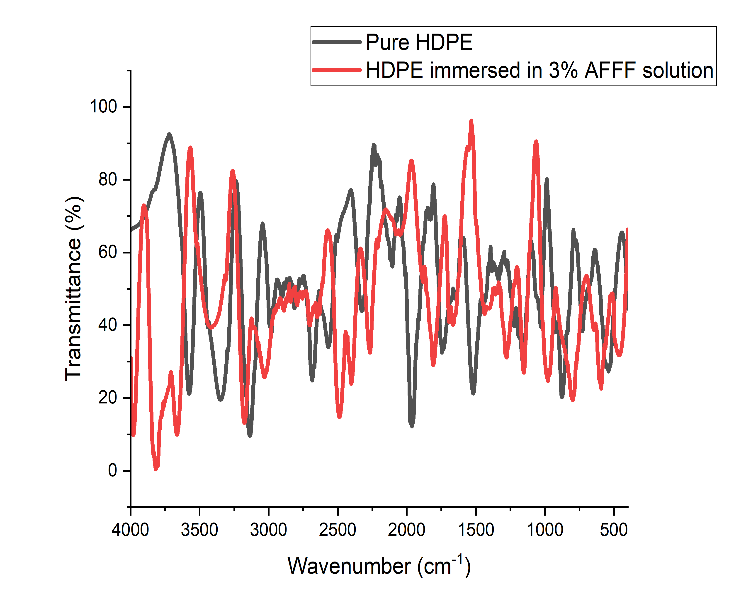
\includegraphics[height=6cm, width=\textwidth]{pure_hdpe_ftir_spectra.png}
    \caption{}
\end{subfigure}
\begin{subfigure}{.45\textwidth}
    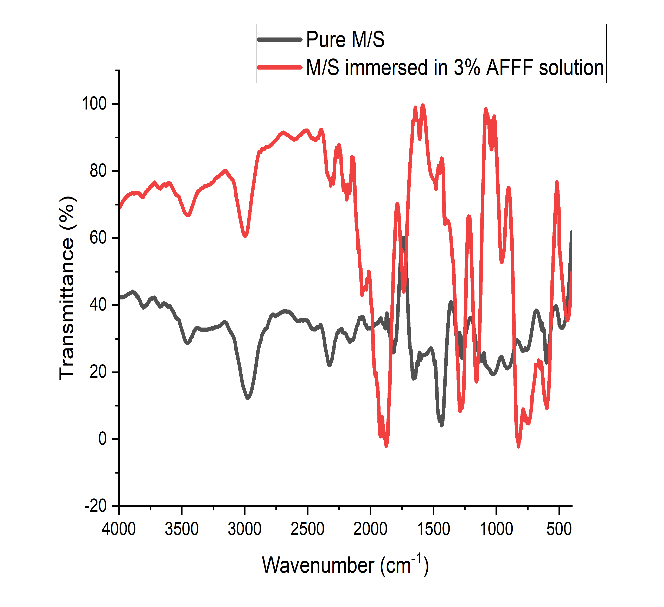
\includegraphics[height=6cm, width=\textwidth]{pure_ms_ftir_spetra.png}
    \caption{}
\end{subfigure}
\begin{subfigure}{.45\textwidth}
    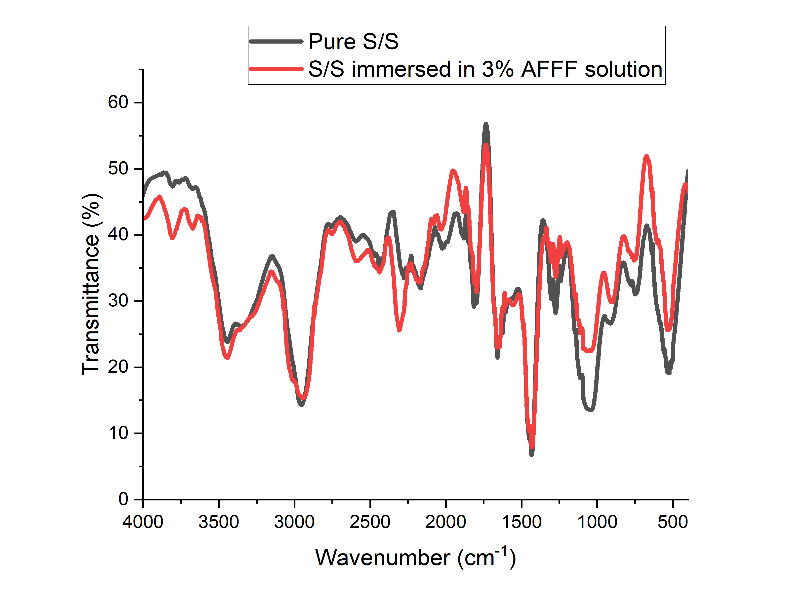
\includegraphics[width=\textwidth]{pure_ss_ftir_spectra.png}
    \caption{}
\end{subfigure}

\caption{FTIR spectra, comparing various materials.}
\label{ch5:figure:materials}
\end{figure}

\section{Transmission Electron Microscopy (TEM)}
The JEOL JEM-1010 TEM used for the present study is equipped with highly integrated technology. The 40kV to 100kV operating voltage range is suitable for applications in material science. Because of its low operating voltage and unique objective pole piece design, the JEM-1010 is a TEM with outstanding contrast \cite{krimm1986vibrational}. Additionally, it has a 2k x 2k AMT CCD camera for taking digital images. The TEM was able to provide overall particle shape, large variety of particles and visual overall of the particle shape of the AFFF solution samples using the high resolution (HR) and electron diffraction imaging.  
The TEM images of pure AFFF solution are shown in Figure \ref{ch5:figure:pure_afff_images}. These will be utilized as a benchmark and will be compared to the immersed solution to observe any critical particle changes. All the samples depict the HR and electron diffraction images in various parts. This was done to understand the overall particle shape of the solution before making any conclusions. 

\begin{figure}[H]
\centering

\begin{subfigure}{.45\textwidth}
    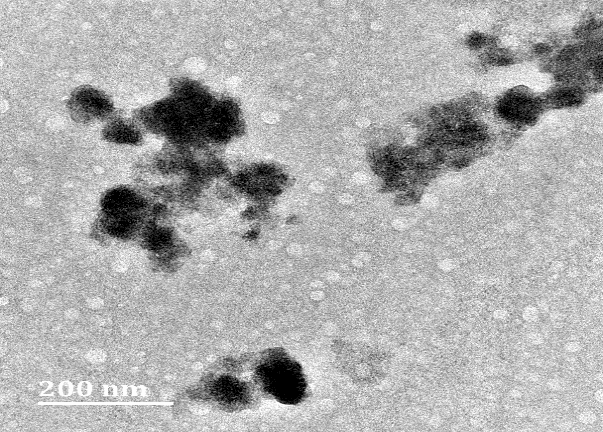
\includegraphics[height=5.3cm, width=\textwidth]{diffraction_image_1.png}
\end{subfigure}
\hspace{-1em}
\begin{subfigure}{.45\textwidth}
    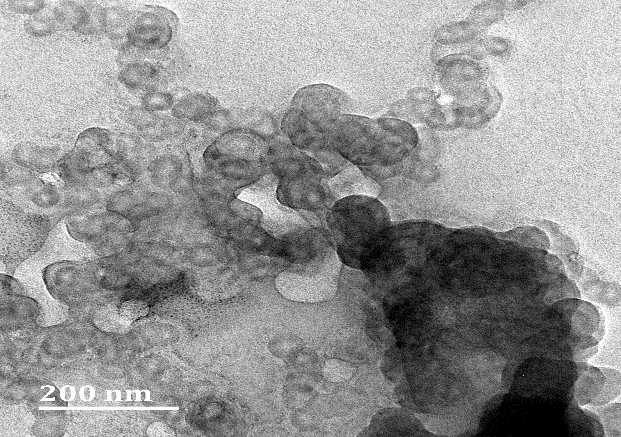
\includegraphics[height=5.3cm, width=\textwidth]{diffraction_image_2.png}
\end{subfigure}
\par\bigskip
\begin{subfigure}{.45\textwidth}
    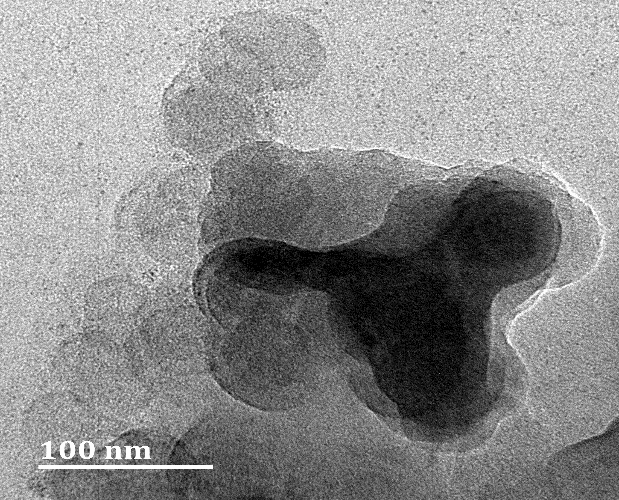
\includegraphics[height=6cm, width=\textwidth]{diffraction_image_3.png}
\end{subfigure}
\hspace{-1em}
\begin{subfigure}{.45\textwidth}
    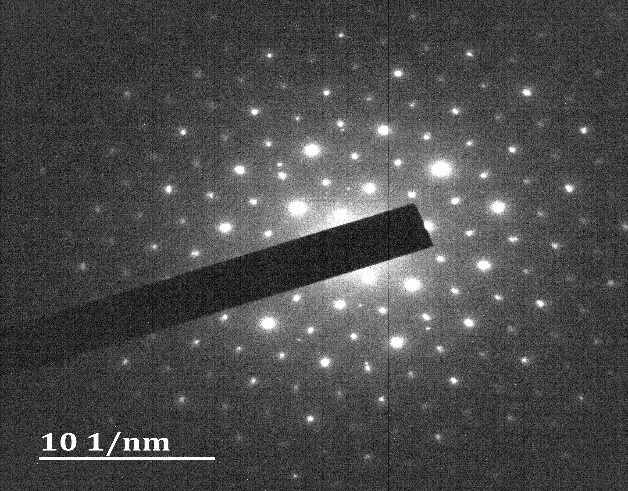
\includegraphics[height=6cm, width=\textwidth]{diffraction_image_4.png}
\end{subfigure}

\caption{HR (a-c) and electron diffraction images (d) of pure AFFF solution.}
\label{ch5:figure:pure_afff_images}
\end{figure}

It can be observed from Figure \ref{ch5:figure:pure_afff_images} (d) that the electron diffraction image of pure AFFF solution provides numerous spot that are aligned in a particular direction. This is a demonstration that the solution in a pure state has a single crystalline structure. This shows that the solution has uniform property characteristics and is more stable in its pure form \cite{coates1996interpretation}.  Moreover, Figure \ref{ch5:figure:pure_afff_images} (a-c) reveal that the particles of pure AFFF solution are scattered along the solution. This might be caused by the collision of two or more repelling particles within the solution \cite{bellamy1980infrared}. Figure \ref{ch5:figure:mild_steel_images} - \ref{ch5:figure:hdpe_images} depict the HR and electron diffraction images when various materials were immersed in AFFF solution. 
  
\begin{figure}[H]
\centering

\begin{subfigure}{.45\textwidth}
    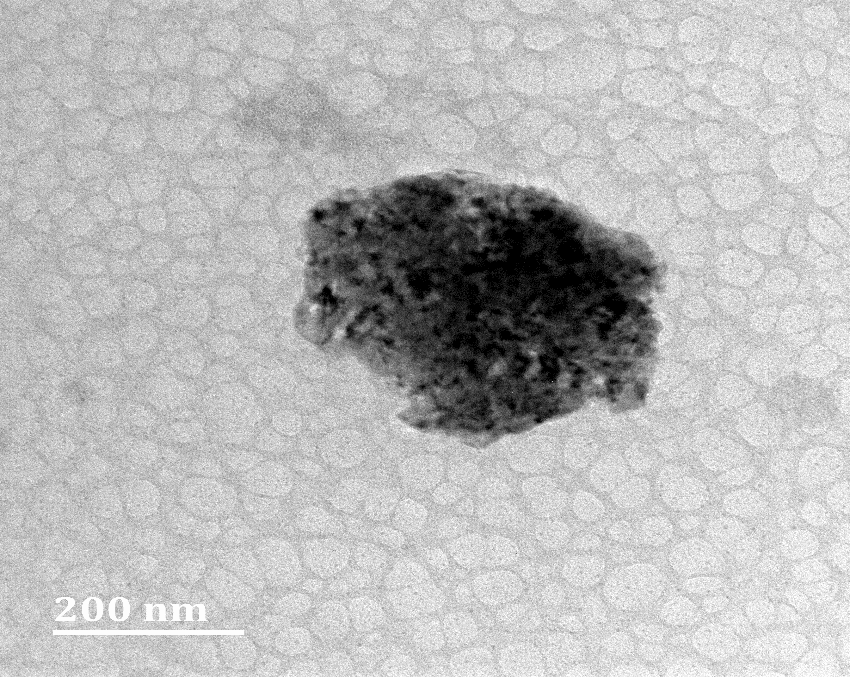
\includegraphics[height=6cm, width=\textwidth]{diffraction_image_5.png}
\end{subfigure}
\hspace{-1em}
\begin{subfigure}{.45\textwidth}
    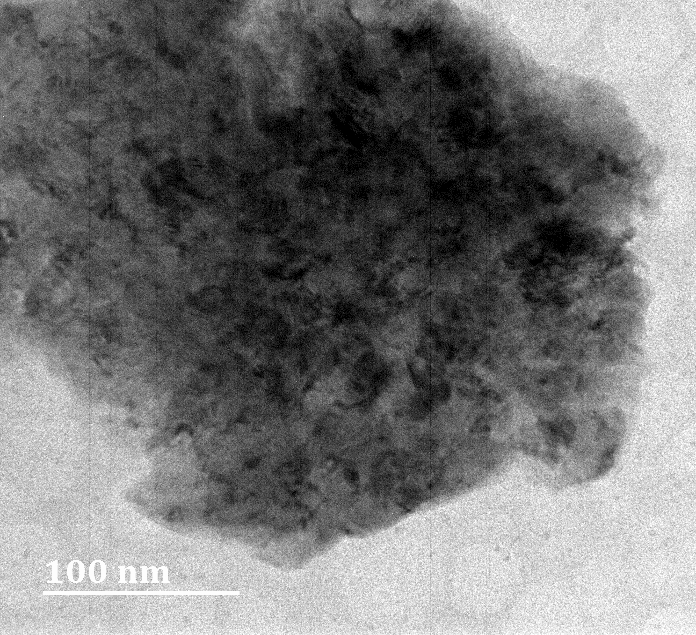
\includegraphics[height=6cm, width=\textwidth]{diffraction_image_6.png}
\end{subfigure}
\par\bigskip
\begin{subfigure}{.45\textwidth}
    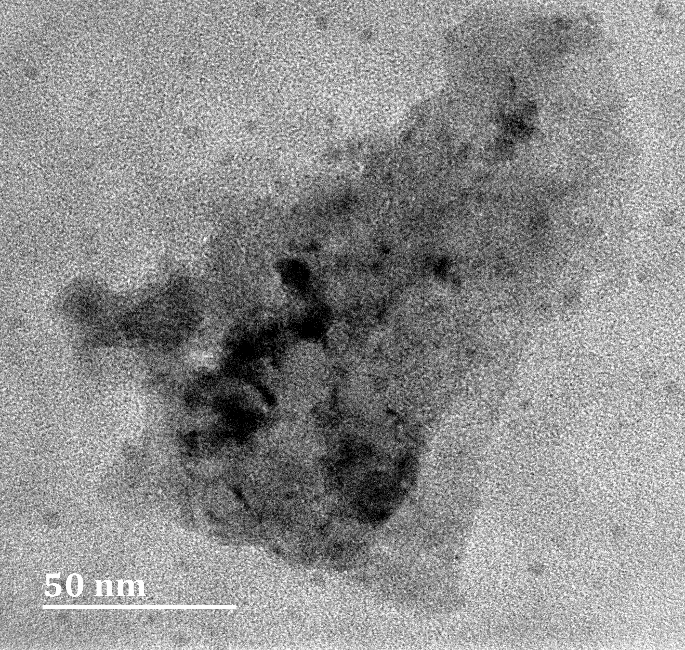
\includegraphics[height=6cm, width=\textwidth]{diffraction_image_7.png}
\end{subfigure}
\hspace{-1em}
\begin{subfigure}{.45\textwidth}
    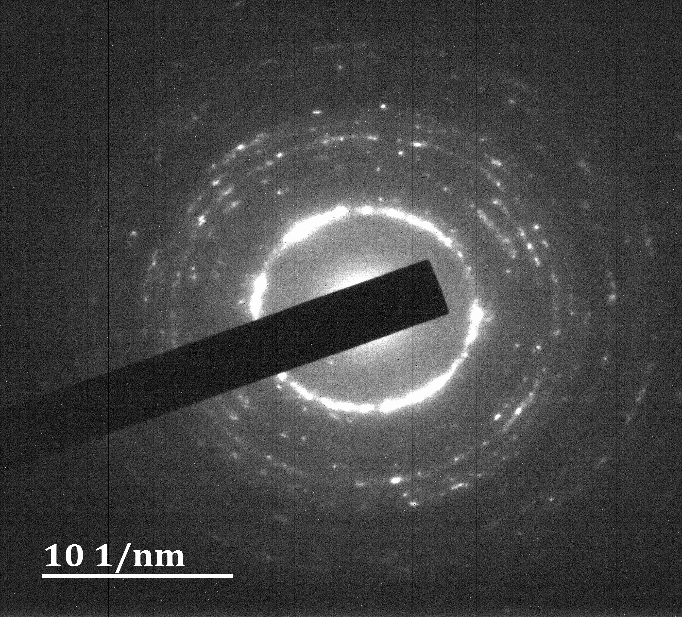
\includegraphics[height=6cm, width=\textwidth]{afff_solution_immersed_in_mild_steel.png}
\end{subfigure}

\caption{HR (a-c) and electron diffraction images (d) of AFFF solution immersed in mild steel.}
\label{ch5:figure:mild_steel_images}
\end{figure}

\begin{figure}[H]
\centering

\begin{subfigure}{.45\textwidth}
    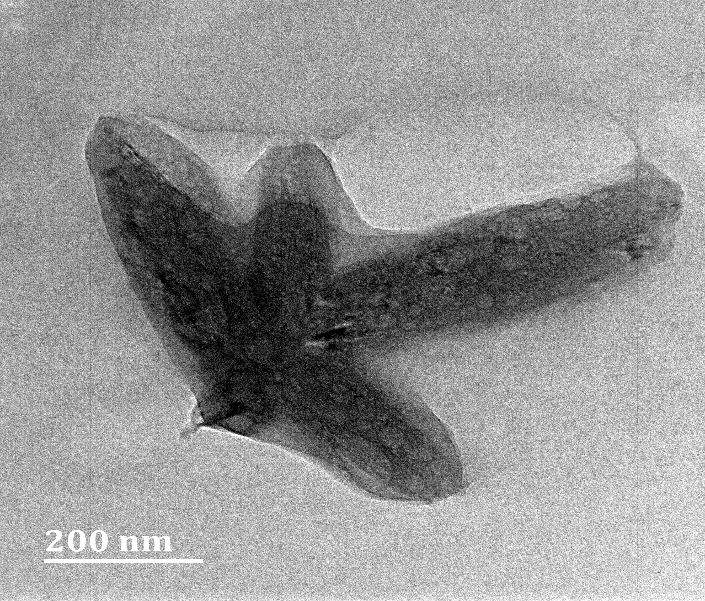
\includegraphics[height=6cm, width=\textwidth]{diffraction_image_8.png}
\end{subfigure}
\hspace{-1em}
\begin{subfigure}{.45\textwidth}
    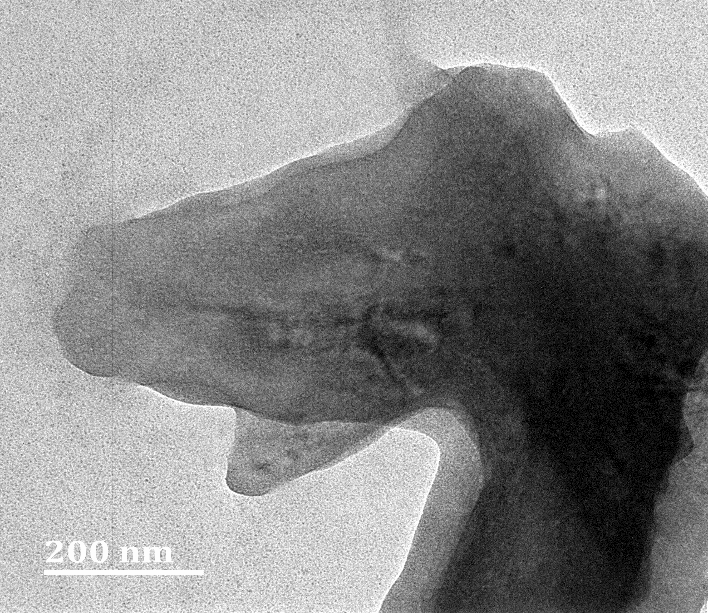
\includegraphics[height=6cm, width=\textwidth]{diffraction_image_9.png}
\end{subfigure}
\par\bigskip
\begin{subfigure}{.45\textwidth}
    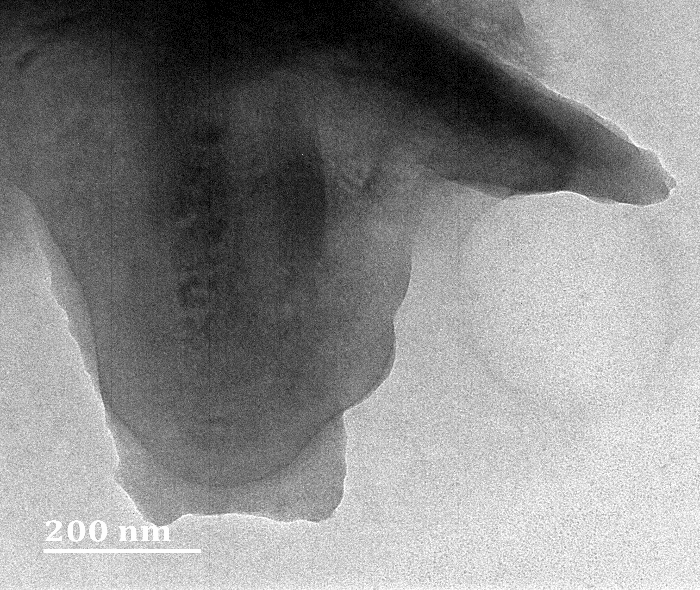
\includegraphics[height=6cm, width=\textwidth]{diffraction_image_10.png}
\end{subfigure}
\hspace{-1em}
\begin{subfigure}{.45\textwidth}
    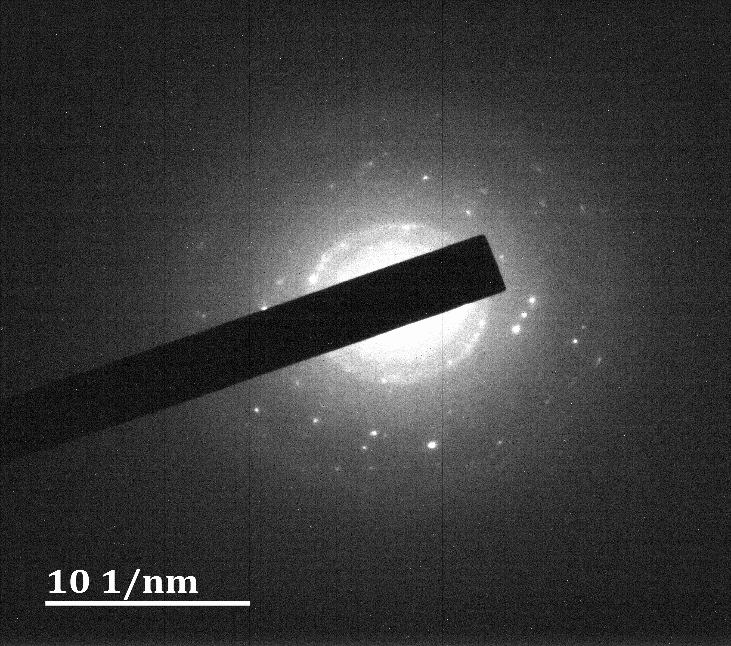
\includegraphics[height=6cm, width=\textwidth]{afff_solution_immersed_in_stainless_steel.png}
\end{subfigure}

\caption{HR (a-c) and electron diffraction images (d) of AFFF solution immersed in stainless steel.}
\label{ch5:figure:stainless_steel_images}
\end{figure}

\begin{figure}[H]
\centering

\begin{subfigure}{.45\textwidth}
    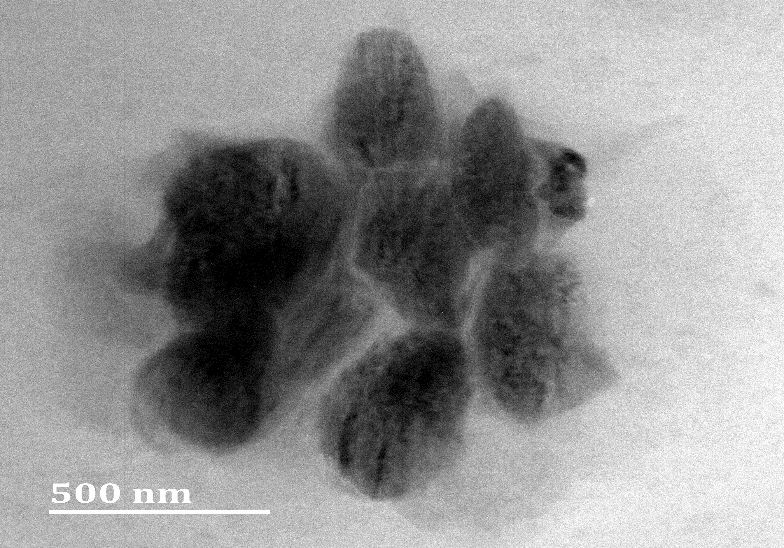
\includegraphics[height=5.5cm, width=\textwidth]{diffraction_image_11.png}
\end{subfigure}
\hspace{-1em}
\begin{subfigure}{.45\textwidth}
    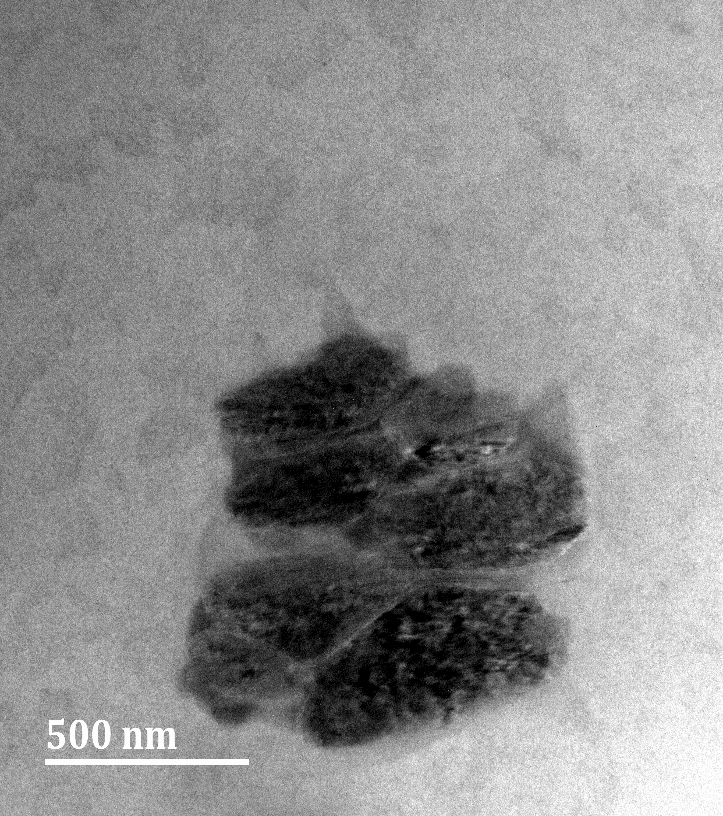
\includegraphics[height=5.5cm, width=\textwidth]{diffraction_image_12.png}
\end{subfigure}
\par\bigskip
\begin{subfigure}{.45\textwidth}
    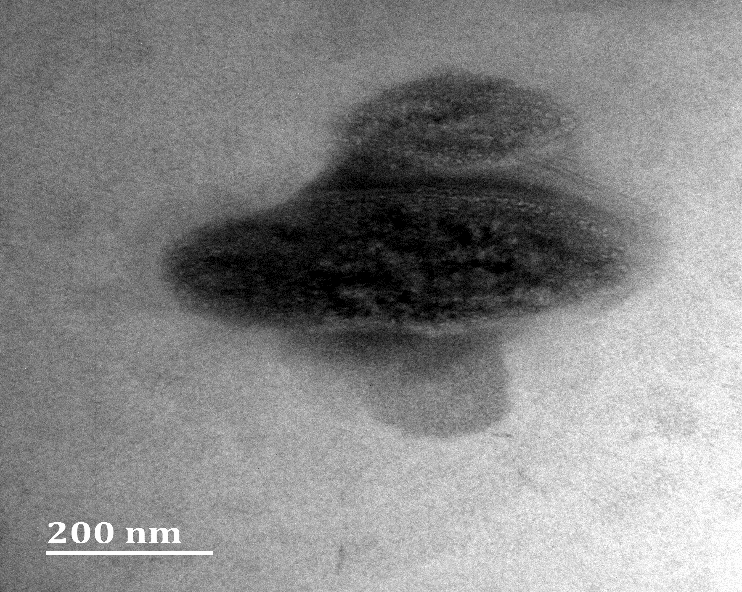
\includegraphics[height=5.5cm, width=\textwidth]{diffraction_image_13.png}
\end{subfigure}
\hspace{-1em}
\begin{subfigure}{.45\textwidth}
    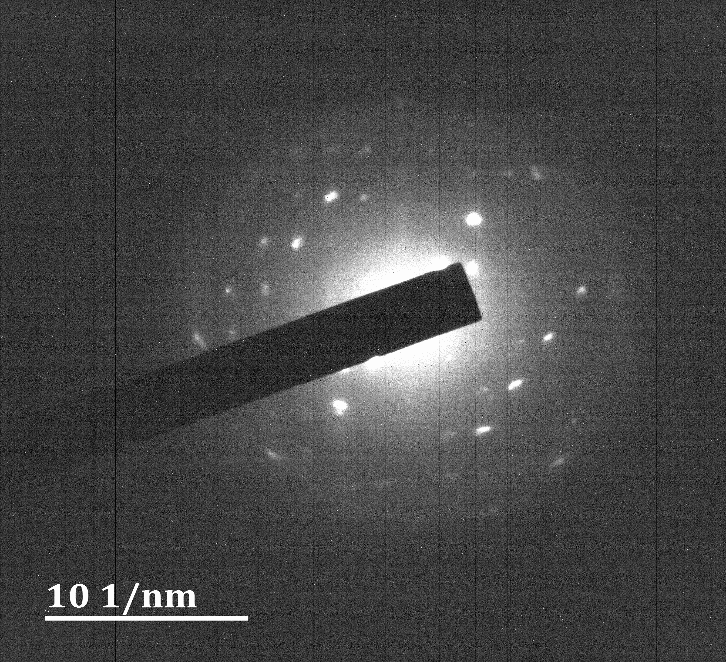
\includegraphics[height=5.5cm, width=\textwidth]{afff_solution_in_hdpe.png}
\end{subfigure}

\caption{HR (a-c) and electron diffraction images (d) of AFFF solution immersed in HDPE.}
\label{ch5:figure:hdpe_images}
\end{figure}

The overall crystal structure and the difference in particle shape for three samples comparing them to pure AFFF sample were studied. Although, the present TEM analysis are not able to provide the precise particle sizes of the samples, it nonetheless provides the significant overall change in crystal structure. Figure \ref{ch5:figure:pure_afff_images} revealed that in a pure state, AFFF solution possesses a single crystalline structure. However, when studying Figure \ref{ch5:figure:mild_steel_images}-\ref{ch5:figure:hdpe_images}, it is observed that the immersed AFFF solution has critically changed to a polycrystalline. This is seen in Figure \ref{ch5:figure:mild_steel_images}-\ref{ch5:figure:hdpe_images} (d) when closely studying the electron diffraction images of these samples. The concentrated circular rounds imply that all these materials are polycrystalline. This is confirmed by the morphology (particles, grains and crystallite), as several grains are observed in Figure \ref{ch5:figure:mild_steel_images}-\ref{ch5:figure:hdpe_images}. These grains are separated by grain boundaries and have random crystallographic orientations. It can be further observed that Figure \ref{ch5:figure:mild_steel_images} has the numerous grains compared to Figure \ref{ch5:figure:stainless_steel_images} and \ref{ch5:figure:hdpe_images}.  Consequently, this implies that most of the crystal structural changes occurred when mild steel was immersed in AFFF solution. 
When comparing the differences topographically (structure and shape), it can be observed in Figure \ref{ch5:figure:pure_afff_images} that the particles for pure AFFF solution are scattered and distributed along the solution. However, when closely observing Figure \ref{ch5:figure:mild_steel_images}-\ref{ch5:figure:hdpe_images} it can been see that the particles for these samples are concentrated in one area, especially in Figure \ref{ch5:figure:mild_steel_images}. This demonstrates that there has been a structural and shape particle change when the materials of interest where immersed in AFFF solution. The alteration in crystal structure and particle shape in AFFF solution complements the shifts in functional groups obtained using the FTIR. An et al \cite{lin1991handbook} experimentally investigated the effect of the particle shape on the viscosity of the liquid. Their results indicated that the spherical particles have lower viscosity and any other particle shape will result in a higher viscosity. In addition, a change in any additive of AFFF solution will affect the foam drainage time. It should be noted that the causes of these alterations are not known as yet. However, conclusive analysis and interpretation are done in section 5.5 and 5.6 using the DLS and elementary analysis to validate the vital information provided by FTIR and TEM.

\section{Dynamic Light Scattering (DLS)}
In this section, the in-depth understanding of the cause of crystal structure and particle shape changes within the AFFF solution and the impact these changes possess on the performance parameters are discussed. This is achieved by evaluating the particle size and particle size distribution of AFFF solution by measurement of the hydrodynamic diameter (Z-average) of any present particles in units of nanometre (nm) using a DLS technique. DLS is a noninvasive technique that depends on the particles moving randomly as a result of collisions with the solvent molecules (Brownian motion). As a result, only particles suspended in a liquid may be categorized \cite{mudunkotuwa2014atr}. The determination of particle size and size distribution is essential because these characteristics have a large effect on the properties of the AFFF solution including the mechanical stability, foaming ability and viscosity \cite{mohamed2017fourier}.

\subsection{Particle size analysis}
Figure \ref{ch5:figure:samples} depict the four samples used during the DLS analysis, where 1,2 and 3 are AFFF solution when mild steel, stainless steel, and HDPE respectively, have been immersed. Sample 4 is a pure AFFF solution for benchmark purposes. Table \ref{ch5:table:sizes} shows the summary of the results for average particle sizes for the four samples in nm.  
  
\begin{figure}[H]
    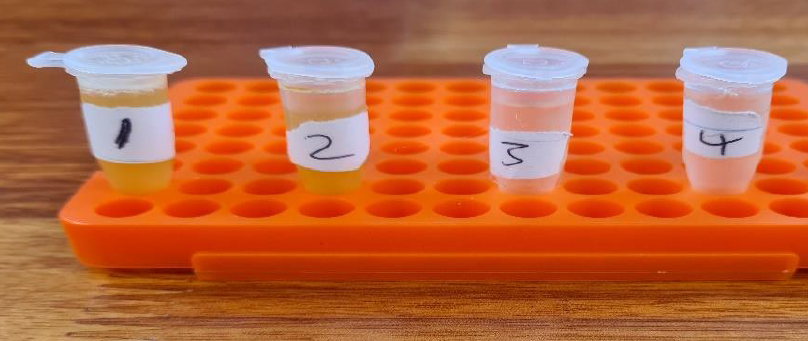
\includegraphics[width=.6\textwidth]{samples_used_during_the_dls_analysis.png}
    \caption{Samples used during the DLS analysis.}
    \label{ch5:figure:samples}
\end{figure}

\begin{table}[H]
\centering
\begin{tabular}{c c}
\hline
\textbf{SAMPLE ID} & \textbf{Z-AVERAGE (D)} \\
\hline
\textbf{1} & 660.7 nm \\
\textbf{2} & 4.892 nm \\
\textbf{3} & 4.036 nm \\
\textbf{4} & 3.586 nm \\
\hline
\end{tabular}

\caption{Summary of average particle sizes.}
\label{ch5:table:sizes}
\end{table}

It can be observed from Table \ref{ch5:table:sizes} that there have been changes in particle size diameter. The pure AFFF solution has an average particle size of 3.586nm, which is a very small particle size. However, when comparing this to sample 2 and 3 it can be observed that there is a slight difference or change. To be precise, the change in Z-average is around 1.306nm at most. At this point, it is not known if these changes are slight in such a way that they do not have any effect on the properties of AFFF solution. Sample 1, in Table \ref{ch5:table:sizes} shows a major change in particle size. Samples 1 has an average particle size of 660.7 nm, which is way above the other three samples by about 655.808 nm at most. This difference is extremely surprising and obviously has some implications. As a matter of fact, larger particles have a gradual diffusion speed than smaller particles. In a fluid, a particle's translational diffusion coefficient and hydrodynamic diameter are related by the Stokes-Einstein equation \cite{lin1991handbook}, as demonstrated by equation \ref{ch5:equation:stokes_einstein}.

\begin{equation}
    D_T=\frac{K_bT}{b\pi \eta R_h}
    \label{ch5:equation:stokes_einstein}
\end{equation}

\noindent Where, \\
$D_T\ is\ the\ transitional\ diffusion\ coefficient\ in\ \nicefrac{m^2}{s}$ \\
$R_H\ is\ the\ hydrodynamic\ radius\ in\ m$ \\
$K_b\ is\ the\ Boltzmann\ constant\ in\ \nicefrac{J}{K}$ \\
$T\ is\ the\ Temperature\ in\ K$ \\
$\eta\ is\ the\ viscosity\ of\ the\ medium\ in\ \nicefrac{Ns}{m^2}$ \\
$b\ is\ the\ constant\ that\ depends\ on\ the\ size\ of\ the\ diffusing\ molecules$ \\

As a matter of fact, for a AFFF stability, a raping diffusion of fluorosurfactant molecules is required. It can be observed from equation \ref{ch5:equation:stokes_einstein} that the rate of diffusion is inversely proportion to the particle size. However, it also depends on the surface area and temperature. For the present study, all the samples were exposed to the same temperature (atmospheric) for equitable comparison. This is a demonstration that once AFFF solution has been in contact with mild steel, it decreases its diffusion rate rapidly and thus decrease the foam ability of AFFF solution.  On the other hand, the Z-average (particle size diameter) results demonstrate that when stainless steel and HDPE have been immersed in AFFF solution there are slight differences in particle diameter when compared to pure AFFF solution. When visually observing the numbers, the difference looks slightly. In contrary, the percentage increase calculations demonstrate a relatively large difference. The percentage increase in particle size for AFFF solution when stainless steel was immersed can be calculated from the basic equation given as: 

\begin{gather}
    \%Increase = \frac{D_s - D_O}{3.586} \times 100 \\ 
    \nonumber \%Increase = \frac{4.892 - 3.586}{3.586}\times 100 \\
    \nonumber \%Increase = 36.419\%
    \label{ch5:equation:stainless_steel}
\end{gather}

Where, \\
$D_s\ is\ the\ particle\ size\ diameter\ of\ sample\ 2\ in\ nm$ \\
$D_O\ is\ the\ particle\ size\ diameter\ of\ sample\ 4\ in\ nm$ \\

Using the same equation, the percentage increase in particle size diameter for AFFF solution when HDPE was immersed is calculated as:  

\begin{gather}
    \%Increase = \frac{D_s - D_O}{D_O} \times 100 \\ 
    \nonumber \%Increase = \frac{4.036 - 3.586}{3.586}\times 100 \\
    \nonumber \%Increase = 12.549\% 
    \label{ch5:equation:hdpe}
\end{gather}
 
Where, \\
$D_s\ is\ the\ particle\ size\ diameter\ of\ sample\ 2\ in\ nm$ \\
$D_O\ is\ the\ particle\ size\ diameter\ of\ sample\ 4\ in\ nm$ \\

It can be seen from equation \ref{ch5:equation:stainless_steel} that the particle size percentage change is 36.419\% when stainless steel was immersed in AFFF solution. This can be regarded as a huge increase since there is more than a quarter (1/4) difference between the two particles. When analyzing equation \ref{ch5:equation:hdpe}, it can be observed that when HDPE was immersed in AFF solution, the particle size has an average change of 12.549 nm. This is a much less percentage compared to 36.419 nm, with a difference of 23.87 nm. Nonetheless, it cannot be guaranteed that it does not influence the foam ability property of AFFF solution.  At this moment, there are still doubts regarding the effects of these materials on AFFF solution. However, the analysis of the particle size distribution (PSD) and element composition will be conducted in sections 5.5.2 and 5.6, respectively, for further validation.

\subsection{Particle size distribution (PSD) analysis} 
DLS is a widely accepted method to evaluate the hydrodynamic size of solution particles. The DLS particle size results can be represented using volume, number and intensity However, as stated in the international standard (ISO 22412:2017), intensity-based results are the most reliable parameters provided by DLS to describe particle size and particle size distribution (PSD) \cite{bellamy1980infrared}. As a consequence, the intensity-based results were opted on the present research work to analyse the PSD of pure AFFF solution and AFFF solution after the three materials were immersed. A comparison in size distribution is then made, in order to understand the influence of each material on the properties of AFFF solution. As a matter of fact, PSD is essential for understanding the chemical and physical properties of a sample. The particles within the AFFF solution have similar size and are relatively uniform. Figure \ref{ch5:figure:pure_afff} depict the PSD curve of the pure AFFF solution by intensity. This PSD curve is used to compare the alteration in PSD of AFFF solution when various materials where immersed. 

\begin{figure}[H]
    \centering
    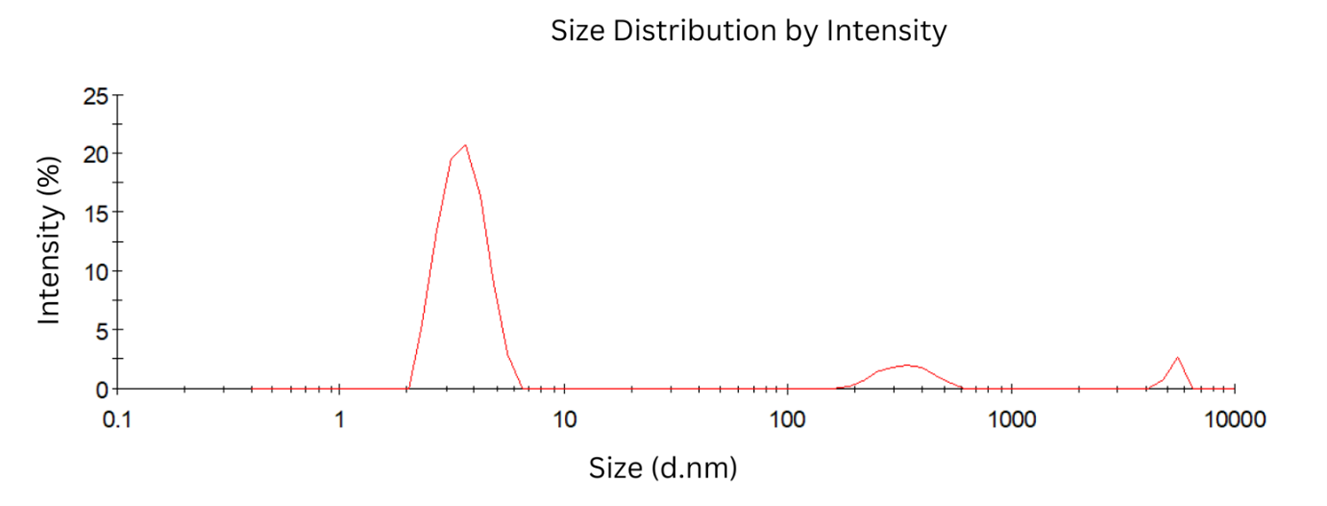
\includegraphics[width=.8\textwidth]{particle_size_distribution_of_pure_afff_solution.png}
    \caption{Particle size distribution of pure AFFF solution.}
    \label{ch5:figure:pure_afff}
\end{figure}

 It can be observed from Figure \ref{ch5:figure:pure_afff} that the particle size distribution curve shows that the peaks are divided into three intensities. As expected, the major peak is at a particle size of 3.586 nm, as previously shown in Table \ref{ch5:table:sizes} and the second and third peaks can be estimated at ~ 350 and 5500 nm, respectively. De la Calle et al. \cite{mudunkotuwa2014atr} studied the particle size distribution of aqueous solution. They demonstrated that the solution with narrow PSD is able to disperse easily. Similarly, it can be seen from Figure \ref{ch5:figure:pure_afff} that the first peak is very narrow. As expected, this is evidence that in a pure state, AFFF solution is able to disperse or spread rapidly over a large surface area. 
 Since this is the intensity based results it is vital to further analyse the amount of scattered light within AFFF solution as it can validate the size of the particles. In Figure \ref{ch5:figure:pure_afff}, the amount of intensity can be estimated to be around 22\%. Based on these findings, it is observed that for AFFF solution, in particular, smaller particles scattered more light. This is further validated by Figure \ref{ch5:figure:stainless_steel}-5.11.
 [ALSO COMMENT ON THE NUMBER OF PEAKS AND RESEARCH MORE ON THE SCATTERED LIGHT what influence does it have, otherwise remove paragraph 2 here]

\begin{figure}[H]
    \centering
    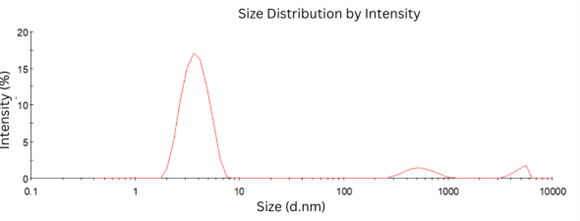
\includegraphics[width=.8\textwidth]{particle_size_distribution_of_afff_solution_when_stainless_steel_was_immersed.png}
    \caption{Particle size distribution of AFFF solution when stainless steel was immersed.}
    \label{ch5:figure:stainless_steel}
\end{figure}

Referring to Figure \ref{ch5:figure:stainless_steel}, it is observed that the AFFF solution possesses 3 peaks. This is precisely the same observation with Figure \ref{ch5:figure:pure_afff}. Unsurprisingly, the main peak can be attributed to a particle size of 4.892 nm. Moreover, it can be seen from Figure \ref{ch5:figure:stainless_steel} that the main peak has a narrow PSD. However, when closely observing it is slightly wider compared to Figure \ref{ch5:figure:pure_afff}. This demonstrates that stainless steel did not cause any critical alteration of PSD within the AFF solution, as it is still able to disperse easily. This is a validation that stainless steel does not influence the spreading ability of AFFF. This further concludes the minor particle size alteration discussed in section 5.5.1 and equation \ref{ch5:equation:stainless_steel} do not have significant impact on the diffusion rate of fluorosurfactant molecules.     
  
\begin{figure}[H]
    \centering
    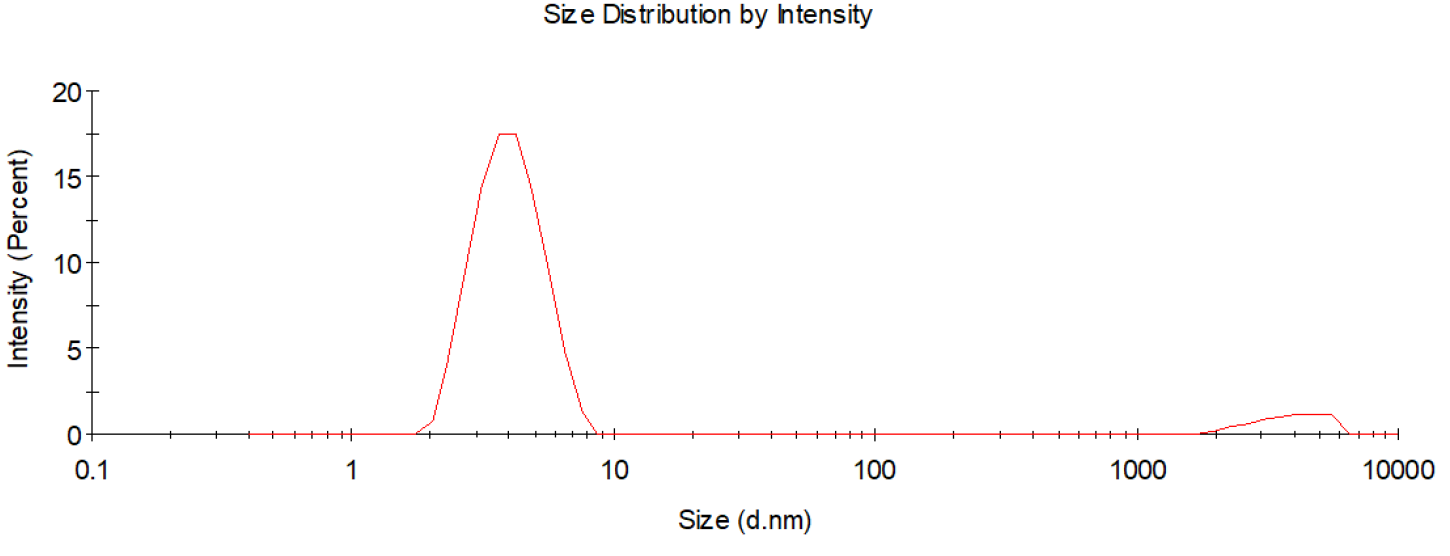
\includegraphics[width=.8\textwidth]{particle_size_distribution_of_afff_solution_when_hdpe_was_immersed.png}
    \caption{Particle size distribution of AFFF solution when HDPE was immersed.}
    \label{ch5:figure:hdpe}
\end{figure}

It can be observed from Figure \ref{ch5:figure:hdpe} that the PSD curve consists of the peaks that are divided into two intensities. This is contrasting when comparing with Figures \ref{ch5:figure:pure_afff} and \ref{ch5:figure:stainless_steel} where the peaks were divided into three intensities. The major peak can be associated with particle size of 4.036 nm, whereas the other peak can be estimated at ~ 5000 nm. When observing the broadness of the major peak, it can be noticed that it is wider than the peak in Figure \ref{ch5:figure:pure_afff} and almost the same size as Figure \ref{ch5:figure:stainless_steel}. However, this can be relatively regarded as a narrow peak. Moreover, this provides sufficient evidence that HDPE does not alter the PSD within the pure AFFF solution, which suggests that the dispersion rate is not affected. This further concludes that the minor particle size alteration discussed in section 5.5.1 and equation \ref{ch5:equation:hdpe} do not have significant impact on the diffusion rate of fluorosurfactant molecules.    
  
\begin{figure}[H]
    \centering
    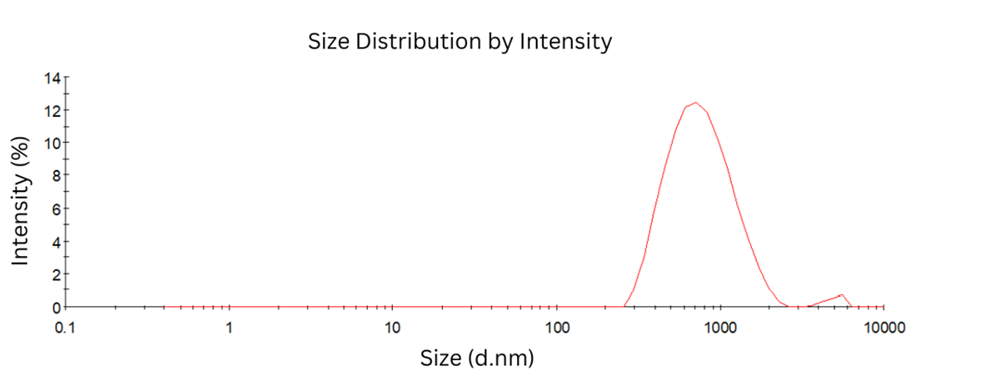
\includegraphics[width=.8\textwidth]{particle_size_distribution_of_afff_solution_when_mild_steel_was_immersed.png}
    \caption{Particle size distribution of AFFF solution when mild steel was immersed.}
    \label{ch5:figure:mild_steel}
\end{figure}

Surprisingly, Figure \ref{ch5:figure:mild_steel} depicts a distinct PSD compared to Figure \ref{ch5:figure:pure_afff}-\ref{ch5:figure:hdpe}. It can be observed that Figure \ref{ch5:figure:mild_steel} reveals peaks that are divided into two intensities. These peaks can be associated with particle size of 660.7 nm, whereas the other peak can be estimated at ~ 5500 nm.  Due to large difference in sizes of these two peaks, they can be generally regarded as major and minor peaks, respectively.  It is interesting to note that Figure \ref{ch5:figure:mild_steel} possesses a wide major peak compared to all previous peaks illustrated in Figure \ref{ch5:figure:pure_afff}-\ref{ch5:figure:hdpe}. This is an indication that there has been a sensitive reaction between mild steel and AFFF solution. Moreover, this demonstrates that the spreading ability of the solution has been reduced. This could be caused by several parameters, such as the increase in viscosity causing the solution to be slightly thicker. However, it is well known that viscosity is largely dependent on the shape of the particles, where any deviation from spherical shape of the particle results in an increase in viscosity \cite{klein2011transmission}. Nevertheless, it is noticed in Figure \ref{ch5:figure:mild_steel} that the PSD can have a slight impact on the spreading capability of the aqueous concentrate.

\section{Wet chemical analysis}
As aforementioned, the ICP-AES was used to identify both the amounts and major concentrations of elements within the exposed AFFF concentrate and benchmark these with the standard quantities and qualities. The alterations in elements or composition can immensely affect the properties, hence the performance of AFFF during the firefighting circumstances. The concrete results are provided in this section, and conclusive information is drawn regarding the severity of mild steel, stainless steel, and HDPE on the performance parameters of AFFF. In addition, the elementary results are more reliable as they provide the precise elements that are present within the AFFF concentrate before and after the materials were immersed. Thus, they validate the previous results of the analyses conducted using FTIR, TEM, and DLS.

\subsection{Elemental componsition analysis}
For the purpose of the present research, the elements were analyzed based on the importance of the role they possess within the AFFF concentrate. To begin with, AFFF is water-based and commonly contains a hydrocarbon-based surfactant such as sodium alkyl sulfate. They discovered that the presence of sodium and sulphur within these fluids is responsible for the stable foam formation. Xiaoyang Yu et al. \cite{yu2020formation} studied the formation of stable aqueous foams. They experimentally demonstrated that the presence of sodium and sulphur within the aqueous solution is responsible for the stable foam formation. As a matter of fact, for stable foam formation, there must be less surface tension in the water. This is mostly accomplished by increasing the sodium alkyl sulfate concentration. As a consequence, sodium and sulphur were the primary elements of interest. Other elements were also analyzed at a later stage, and their impacts on the performance parameter of AFFF were concisely discussed. Table \ref{ch5:table:chemical_elements_1} depicts the elemental composition results of the pure AFFF concentrate and the other when mild steel, stainless steel, and HDPE were immersed. The entire elemental composition results are depicted in Figure F.1 and F.2 in the appendices for validation purposes.

\newcolumntype{Y}{>{\centering\arraybackslash}X}

\begin{table}[H]
\caption{Chemical elements of AFFF concentrate.}

\begin{tabularx}{\textwidth}{*{6}{Y}}
\hline
Element & Chemical symbol & \multicolumn{4}{c}{Composition in PPM} \\
& & \multicolumn{4}{c}{Sample ID:} \\
\hline
& & 1 & 2 & 3 & 4 \\
Sodium & Na & 2302 & 2332 & 2349 & 2354 \\
Sulphur & S & 92 & 89 & 94.2 & 94.7 \\
\hline
\end{tabularx}

\label{ch5:table:chemical_elements_1}
\end{table}

Referring to Table \ref{ch5:table:chemical_elements_1}, samples 1-3 are the AFFF concentrate after mild steel, stainless steel, and HDPE were immersed, respectively, with sample 4 being the pure AFFF concentrate. From Table 4, it can be observed that in a pure state, AFFF concentrate has 2354 and 94.7 parts per million (ppm) of sodium and sulphur, respectively. When observing closely, it is seen that the sodium element decreases gradually from sample 4-1. To be precise, the sodium element is reduced by 5, 22, and 52 ppm, respectively, from the pure AFFF concentrate. This indicates that the sodium composition of the AFFF concentrate is reduced when it is exposed to the materials of interest. Moreover, it can be observed that the amount of reduction in sodium is diverse in all samples. This further demonstrates that the severity of the effects caused by the materials on the foam’s stability varies greatly.
Similar occurrences can be observed with sulphur. Referring to Table \ref{ch5:table:chemical_elements_1}, it is observed that the elemental composition of sulphur in pure AFFF decreases when it reacts with various materials. Consequently, it is evident that the reaction of the three materials with the AFFF concentrate reduces the surfactants (sodium alkyl sulfate). This increases the surface tension of the water within the concentrate, reducing the stability of the foam. Moreover, it can be seen that the sodium alkyl sulphate was immensely reduced when the AFFF concentrate was in contact with mild steel (Sample 1). These findings correlate with FTIR analyses, which confirmed the presence of isothiocyanate N=C=S stretching on the triple bond region at bands 2056 and 2060. This functional group confirmed the presence of sulphur in the AFFF concentrate when HDPE and stainless steel were immersed, but sulfur did not appear in the AFFF concentrate when mild steel was immersed.
In addition, the elementary findings further correlate with the gradual diffusion rate of surfactants due to large particles discussed in 5.5.1. These findings are evidence that stainless steel and HDPE have a minimal effect on the foam ability and foam stability of AFFF. They further demonstrate that mild steel has a severe impact on the two performance parameters of AFFF due to the chemical elements’ reactions with surfactants. However, further studies should be conducted to determine the precise causes of the negative effects of these materials, as this research is limited on the impacts or effects of the materials in AFFF concentrate. In this way, it will be uncomplicated to optimize these materials in such a way that they are compatible with the AFFF concentrate.
The ICP-AES used for the present research was not able to detect organic compounds. However, the functional groups revealed by FTIR spectra were sufficient to provide the key variations of the elements within the AFFF concentrate. The shifting of C-F stretch observed in Section \ref{ch5:table:chemical_elements_1} confirmed that the materials of interest also affect the fluorine content that is present within the PFAS in AFFF concentrate. This alteration of fluorine is a huge setback for the performance parameters of AFFF. As a matter of fact, PFAS are responsible for forming an aqueous film on fire fuels, which effectively suffocates them by creating a barrier to any oxygen and cooling them to prevent hot fuels from reigniting \cite{hinnant2020characterizing}. Consequently, the alteration of fluorine within the AFFF concentrate greatly reduces the blanketing capabilities during firefighting. It is well known that PFAS are harmful to the environment and humans (carcinogenic). However, the AFFF is primarily chosen for its effective extinguishing capabilities due to PFAS. This implies that any alteration of fluorine within the AFFF concentrate yields unfavorable outcomes. Other vital elements that influence the performance of AFFF are listed in Table \ref{ch5:table:chemical_elements_2} and concisely discussed.

\begin{table}[H]
\caption{Chemical elements of AFFF concentrate}

\begin{tabularx}{\textwidth}{*{6}{Y}}
\hline
Element & Chemical symbol & \multicolumn{4}{c}{Composition in PPM} \\
& & \multicolumn{4}{c}{Sample ID:} \\
\hline
& & 1 & 2 & 3 & 4 \\
Aluminium & Al & 0.9 & 0.2 & 0.5 & 1.1 \\
Calcium & Ca & 46 & 07 & 10 & 6.9 \\
Iron & Fe & 132 & 58 & 3.7 & 2.5 \\
Potassium & K & 04 & 03 & 2.8 & 2.4 \\
Magnesium & Mg & 27 & 03 & 2.4 & 2.3 \\
Silicon & Si & 07 & 07 & 11 & 10.6 \\
\hline
\end{tabularx}

\label{ch5:table:chemical_elements_2}
\end{table}

Referring to Table \ref{ch5:table:chemical_elements_2}, it is noticed that the iron content observed in pure AFFF concentrate increased when various materials were immersed. Initially, the iron concentration was 2.5 ppm; it then increased to 3.7 ppm, 58 ppm, and 132 ppm when HDPE, stainless steel, and mild steel were immersed, respectively. In general, the increase in the iron element predominantly implies the degradation or wearing of the material \cite{mcarthur2004engineering}. Consequently, this demonstrates that mild steel degrades immensely when in contact with the AFFF concentrate, as the iron element increases by 129.5 ppm. This is evidence that there is a severe reaction between AFFF concentrate and mild steel. The obvious reason for this could be the initiation of corrosion in mild steel when it was first exposed to the environmental conditions prior to immersion in AFFF concentrate. On the other hand, HDPE and stainless steel underwent a similar process, with severity being the major difference. The iron element increased by 1.2 and 55.5 ppm when HDPE and stainless steel reacted with AFFF concentrate, respectively.
The other elements, such as calcium, potassium, and magnesium, are typically water additives. However, the concern is the variation of these elements across the four samples. Subsequently, the degradation of the materials made the AFFF concentrate impure, possibly influencing its firefighting capabilities. This is drawn from a visual observation of the various AFFF concentrates during the post-experimental work. Figure \ref{ch5:figure:pureness} depicts the state of pureness of AFFF concentrate after the immersion of materials.
 
\begin{figure}[H]
    \centering
    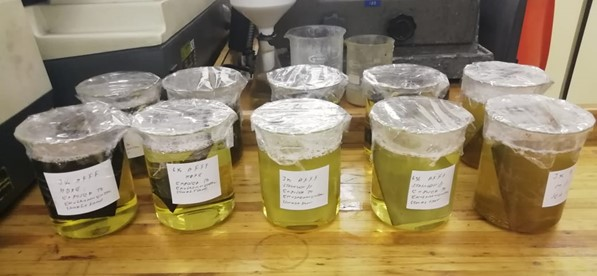
\includegraphics[width=\textwidth]{pureness_of_immersed_afff.jpg}
    \caption{Pureness of AFFF concentrate after immersion of the materials.}
    \label{ch5:figure:pureness}
\end{figure}

It can be observed from Figure \ref{ch5:figure:pureness} that the pureness of the samples varies greatly. Samples (a-b) are AFFF concentrates when HDPE was immersed, and samples (c-d) are when stainless steel was immersed. It is clear from these samples that there was no significant degradation of the materials immersed. This is because the AFFF concentrate was able to maintain its pure yellowish color during the interaction with these materials. However, when observing closely, it is noticed that samples a–b are purer than samples c–d. This is evidence that stainless steel also underwent the degradation process due to the increase of iron by 55.5 ppm, as suggested by Table \ref{ch5:table:chemical_elements_2}. In contrast, sample (e) is the AFFF concentrate when mild steel was immersed. It can be visually observed that mild steel is immensely degraded when it interacts with AFFF concentrate. The AFFF concentrate's transition from a yellowish to a brownish color serves as visual evidence of this. This is further justified by the large increase in iron of 129.5 ppm observed in Table \ref{ch5:table:chemical_elements_2}. Although the precise performance parameters affected by this degradation cannot be concluded, the reaction between mild steel and AFFF concentrate remains severe.

\section{Conclusion}
This chapter documented the results obtained using the FTIR, TEM, DLS, and ICP-AES instruments. Tests were conducted to determine the impact of mild steel, stainless steel, and HDPE on the performance parameters of AFFF. The analyses entangled the function groups, particle shape, and size distribution, as well as the elemental composition of AFFF concentrate. Most of the tests conducted can be classified as successes with regards to reliability. For each test, the results are illustrated in the form of either graphs, pictures, calculations, or tables, as well as a discussion of any relevant observations or concerns arising from the results. AFFF performance parameters such as foam ability, foam stability, surface tension, foam drainage, and viscosity were all found to be statistically significant during the analyses. Among the three materials tested, mild steel was found to have the greatest impact on AFFF performance parameters. While stainless steel was the second ‘severe’ material, HDPE was the compatible material with only the ESC concerns.